\documentclass[aspectratio=169,9pt]{beamer}
\usetheme{default}
\usecolortheme{default}

\usepackage[T1]{fontenc}
\usepackage{lmodern}
\usepackage{booktabs}
\usepackage{array}
\usepackage{colortbl}
\usepackage{xcolor}
\usepackage{tikz}
\usepackage{graphicx}
\usepackage{enumitem}
\usetikzlibrary{shapes.geometric,arrows.meta,positioning,calc,shadows}

% ── Colors (light theme) ──
\definecolor{titlebg}{HTML}{1E3A5F}
\definecolor{blue1}{HTML}{1565C0}
\definecolor{blue2}{HTML}{1976D2}
\definecolor{bluelight}{HTML}{E3F2FD}
\definecolor{orange1}{HTML}{E65100}
\definecolor{orangelight}{HTML}{FFF3E0}
\definecolor{green1}{HTML}{2E7D32}
\definecolor{greenlight}{HTML}{E8F5E9}
\definecolor{purple1}{HTML}{6A1B9A}
\definecolor{purplelight}{HTML}{F3E5F5}
\definecolor{deepblue}{HTML}{4527A0}
\definecolor{brown1}{HTML}{5D4037}
\definecolor{brownlight}{HTML}{EFEBE9}
\definecolor{txtmain}{HTML}{212121}
\definecolor{txtsub}{HTML}{616161}
\definecolor{txtfaint}{HTML}{9E9E9E}
\definecolor{accent}{HTML}{FF6F00}
\definecolor{divider}{HTML}{E0E0E0}

% ── Beamer settings ──
\setbeamercolor{background canvas}{bg=white}
\setbeamercolor{normal text}{fg=txtmain}
\setbeamertemplate{navigation symbols}{}
\setbeamertemplate{frametitle}{}
\setbeamertemplate{footline}{}

% ── Macros ──
\newcommand{\sheader}[3]{%
  \par\smallskip
  \colorbox{#1}{\parbox{\dimexpr\linewidth-2\fboxsep}{\centering\strut\textbf{\textcolor{white}{\footnotesize #2}}\strut}}%
  \par\vspace{#3}%
}

\newcommand{\feat}[1]{\textcolor{txtsub}{\ttfamily\fontsize{6.5}{8}\selectfont #1}}
\newcommand{\flabel}[1]{{\fontsize{7}{9}\selectfont\textbf{\textcolor{blue1}{#1}}}}

\begin{document}

% ════════════════════════════════════════════════════════════════
% SLIDE 1: Data Cleaning (7-Step Pipeline)
% ════════════════════════════════════════════════════════════════
{
\begin{frame}[shrink=14]

% Title bar

\begin{tikzpicture}
\fill[titlebg,rounded corners=3pt] (0,0) rectangle (\textwidth,1.3cm);
\node[anchor=center,font=\Large\bfseries,text=white] at (0.5\textwidth,0.8cm)
  {Data Cleaning --- 7-Step Pipeline};
\node[anchor=center,font=\small,text=white!80] at (0.5\textwidth,0.3cm)
  {1,496,208 raw rows $\times$ 25 cols~~\textbullet~~\texttt{src/data\_cleaner.py}~~\textbullet~~Sequential stages with \texttt{CleaningReport} tracking};
\end{tikzpicture}

\vspace{4pt}

% Table
\centering
\renewcommand{\arraystretch}{1.4}
\resizebox{\textwidth}{!}{%
\fontsize{8}{10.5}\selectfont
\begin{tabular}{@{} >{\centering}p{0.5cm} l l p{6.2cm} >{\raggedleft\arraybackslash}p{2.0cm} @{}}
\toprule
\textbf{Step} & \textbf{Function} & \textbf{Action} & \textbf{Detail} & \textbf{Rows After} \\
\midrule
\cellcolor{bluelight}\textbf{1}
  & \texttt{drop\_nan\_simscode}
  & Remove null join keys
  & Drops rows where \texttt{simsCode} is NaN; converts float\,$\to$\,int\,$\to$\,str
  & 1{,}478{,}640 \\
\cellcolor{bluelight}\textbf{2}
  & \texttt{exclude\_utilities}
  & Drop OIL28SEC
  & 100\% zero readings --- no signal; constant \texttt{EXCLUDED\_UTILITIES}
  & 1{,}469{,}856 \\
\cellcolor{bluelight}\textbf{3}
  & \texttt{exclude\_unmatched\_buildings}
  & Drop codes 8, 43, 93
  & No matching metadata in SIMS; constant \texttt{EXCLUDED\_SIMSCODES}
  & 1{,}465{,}464 \\
\cellcolor{orangelight}\textbf{4}
  & \texttt{apply\_hard\_caps}
  & Sensor-fault outlier removal
  & Per-utility caps: ELEC/HEAT/COOL~10k; GAS~50k; STEAM~1M
  & 1{,}460{,}283 \\
\cellcolor{greenlight}\textbf{5}
  & \texttt{impute\_short\_gaps}
  & Fill gaps $\leq$\,8 intervals
  & Groups by \texttt{(meterId, simsCode, utility)}; ffill then bfill. \textit{112 cells filled}
  & 1{,}460{,}283 \\
\cellcolor{purplelight}\textbf{6}
  & \texttt{drop\_dead\_meters}
  & Remove 100\% NaN meters
  & 47 meters where every \texttt{readingValue} is NaN dropped entirely
  & 1{,}391{,}475 \\
\cellcolor{purplelight}\textbf{7}
  & \texttt{drop\_sparse\_meters}
  & Remove $>$\,50\% NaN meters
  & Meters with NaN fraction above \texttt{SPARSE\_THRESHOLD = 0.5}
  & \textbf{1{,}391{,}475} \\
\bottomrule
\end{tabular}%
}

\vspace{8pt}

\begin{columns}[T,totalwidth=\textwidth]

% Left: raw input
\begin{column}{0.48\textwidth}
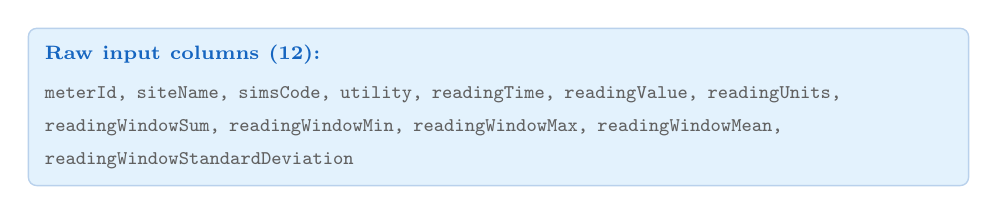
\begin{tikzpicture}
\node[fill=bluelight,rounded corners=3pt,inner sep=6pt,draw=blue1!30,line width=0.5pt,
      text width=0.95\linewidth,align=left] {%
  \fontsize{7}{9}\selectfont
  \textbf{\textcolor{blue1}{Raw input columns (12):}}\\[2pt]
  \textcolor{txtsub}{\ttfamily meterId, siteName, simsCode, utility,
  readingTime, readingValue, readingUnits,
  readingWindowSum, readingWindowMin, readingWindowMax,
  readingWindowMean, readingWindowStandardDeviation}%
};
\end{tikzpicture}
\end{column}

% Right: output
\begin{column}{0.48\textwidth}
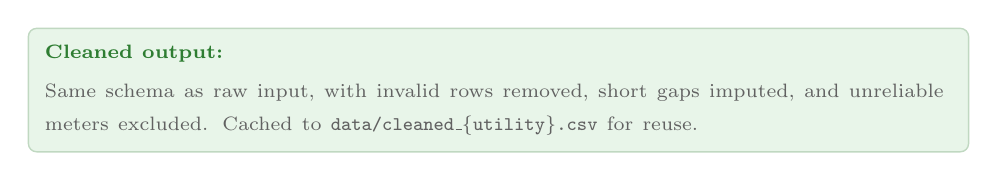
\begin{tikzpicture}
\node[fill=greenlight,rounded corners=3pt,inner sep=6pt,draw=green1!30,line width=0.5pt,
      text width=0.95\linewidth,align=left] {%
  \fontsize{7}{9}\selectfont
  \textbf{\textcolor{green1}{Cleaned output:}}\\[2pt]
  \textcolor{txtsub}{Same schema as raw input, with invalid rows removed,
  short gaps imputed, and unreliable meters excluded.
  Cached to \texttt{data/cleaned\_\{utility\}.csv} for reuse.}%
};
\end{tikzpicture}
\end{column}

\end{columns}

\vspace*{\fill}
{\centering\textcolor{txtfaint}{\fontsize{5.5}{7}\selectfont OSU AI Hackathon --- Team Anarchy~~|~~Strategic Energy Investment Prioritization}\par}

\end{frame}
}


% ════════════════════════════════════════════════════════════════
% SLIDE 2: Data Shape per Utility per Cleaning Step
% ════════════════════════════════════════════════════════════════
{
\begin{frame}

% Title bar

\begin{tikzpicture}
\fill[titlebg,rounded corners=3pt] (0,0) rectangle (\textwidth,1.3cm);
\node[anchor=center,font=\Large\bfseries,text=white] at (0.5\textwidth,0.8cm)
  {Data Shape --- Per Utility After Each Step};
\node[anchor=center,font=\small,text=white!80] at (0.5\textwidth,0.3cm)
  {Row counts by utility type through the 7-step cleaning pipeline};
\end{tikzpicture}

\vspace{6pt}

\centering
\renewcommand{\arraystretch}{1.55}
\resizebox{\textwidth}{!}{%
\fontsize{9}{12}\selectfont
\begin{tabular}{@{} l
    >{\centering\arraybackslash}p{2.2cm}
    >{\centering\arraybackslash}p{2.2cm}
    >{\centering\arraybackslash}p{2.2cm}
    >{\centering\arraybackslash}p{2.2cm}
    >{\centering\arraybackslash}p{2.2cm}
    >{\raggedleft\arraybackslash}p{2.2cm} @{}}
\toprule
\textbf{Step}
  & \textbf{\textcolor{blue1}{Electricity}}
  & \textbf{\textcolor{orange1}{Gas}}
  & \textbf{\textcolor{red!70!black}{Heat}}
  & \textbf{\textcolor{txtsub}{Steam}}
  & \textbf{\textcolor{blue2}{Cooling}}
  & \textbf{Total} \\
\midrule
\cellcolor{bluelight}\textbf{Raw input}
  & 745{,}176 & 238{,}632 & 244{,}488 & 55{,}632 & 200{,}568
  & \textbf{1{,}496{,}208} \\
\cellcolor{bluelight}\textbf{1.}\;drop NaN keys
  & 733{,}464 & 237{,}168 & 240{,}096 & 55{,}632 & 200{,}568
  & 1{,}478{,}640 \\
\cellcolor{bluelight}\textbf{2.}\;exclude utilities
  & 733{,}464 & 237{,}168 & 240{,}096 & 55{,}632 & 200{,}568
  & 1{,}469{,}856 \\
\cellcolor{bluelight}\textbf{3.}\;exclude buildings
  & 729{,}072 & 237{,}168 & 240{,}096 & 55{,}632 & 200{,}568
  & 1{,}465{,}464 \\
\cellcolor{orangelight}\textbf{4.}\;hard caps
  & 727{,}582 & 237{,}036 & 239{,}868 & 54{,}698 & 199{,}635
  & 1{,}460{,}283 \\
\cellcolor{greenlight}\textbf{5.}\;impute gaps
  & 727{,}582 & 237{,}036 & 239{,}868 & 54{,}698 & 199{,}635
  & 1{,}460{,}283 \\
\cellcolor{purplelight}\textbf{6.}\;dead meters
  & 689{,}518 & 232{,}644 & 228{,}156 & 48{,}842 & 190{,}851
  & 1{,}391{,}475 \\
\cellcolor{purplelight}\textbf{7.}\;sparse meters
  & 689{,}518 & 232{,}644 & 228{,}156 & 48{,}842 & 190{,}851
  & \textbf{1{,}391{,}475} \\
\midrule
\textbf{Rows removed}
  & \textcolor{red!70!black}{55{,}658} & \textcolor{red!70!black}{5{,}988} & \textcolor{red!70!black}{16{,}332} & \textcolor{red!70!black}{6{,}790} & \textcolor{red!70!black}{9{,}717}
  & \textcolor{red!70!black}{\textbf{104{,}733}} \\
\textbf{Retention}
  & \cellcolor{greenlight}\textbf{92.5\%} & \cellcolor{greenlight}\textbf{97.5\%} & \cellcolor{greenlight}\textbf{93.3\%} & \cellcolor{greenlight}\textbf{87.8\%} & \cellcolor{greenlight}\textbf{95.2\%}
  & \cellcolor{greenlight}\textbf{93.0\%} \\
\bottomrule
\end{tabular}%
}% end resizebox

\vspace{10pt}

% Takeaway boxes
\begin{columns}[T,totalwidth=\textwidth]

\begin{column}{0.48\textwidth}
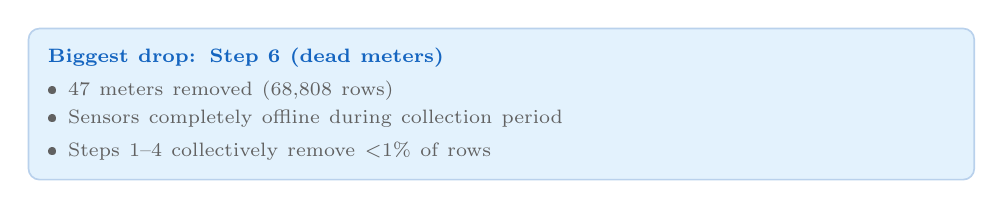
\begin{tikzpicture}
\node[fill=bluelight,rounded corners=4pt,inner sep=7pt,draw=blue1!30,line width=0.6pt,
      text width=0.95\linewidth,align=left] {%
  \fontsize{7.5}{10}\selectfont\textcolor{txtmain}{%
  \textbf{\textcolor{blue1}{Biggest drop: Step 6 (dead meters)}}\\[2pt]
  \textcolor{txtsub}{%
  \textbullet~47 meters removed (68{,}808 rows)\\
  \textbullet~Sensors completely offline during collection period\\
  \textbullet~Steps 1--4 collectively remove $<$1\% of rows}}%
};
\end{tikzpicture}
\end{column}

\begin{column}{0.48\textwidth}
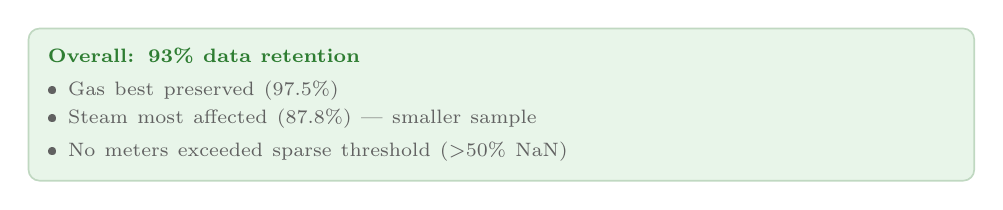
\begin{tikzpicture}
\node[fill=greenlight,rounded corners=4pt,inner sep=7pt,draw=green1!30,line width=0.6pt,
      text width=0.95\linewidth,align=left] {%
  \fontsize{7.5}{10}\selectfont\textcolor{txtmain}{%
  \textbf{\textcolor{green1}{Overall: 93\% data retention}}\\[2pt]
  \textcolor{txtsub}{%
  \textbullet~Gas best preserved (97.5\%)\\
  \textbullet~Steam most affected (87.8\%) --- smaller sample\\
  \textbullet~No meters exceeded sparse threshold ($>$50\% NaN)}}%
};
\end{tikzpicture}
\end{column}

\end{columns}

\vspace*{\fill}
{\centering\textcolor{txtfaint}{\fontsize{5.5}{7}\selectfont OSU AI Hackathon --- Team Anarchy~~|~~Strategic Energy Investment Prioritization}\par}

\end{frame}
}


% ════════════════════════════════════════════════════════════════
% SLIDE 3: XGBoost Models (was Slide 2)
% ════════════════════════════════════════════════════════════════
{
\begin{frame}[shrink=10]

% Title bar using tikzpicture (not overlay)

\begin{tikzpicture}
\fill[titlebg,rounded corners=3pt] (0,0) rectangle (\textwidth,1.3cm);
\node[anchor=center,font=\Large\bfseries,text=white] at (0.5\textwidth,0.8cm)
  {XGBoost Models --- All 5 Utilities};
\node[anchor=center,font=\small,text=white!80] at (0.5\textwidth,0.3cm)
  {ELECTRICITY\;\textbullet\;GAS\;\textbullet\;HEAT\;\textbullet\;STEAM\;\textbullet\;COOLING};
\end{tikzpicture}

\vspace{4pt}

\begin{columns}[T,totalwidth=\textwidth]

% ──── LEFT: Input Features ────
\begin{column}{0.34\textwidth}
\sheader{blue1}{INPUT FEATURES (25)}{2pt}

\flabel{Weather (8)}\\[1pt]
\feat{\textbullet~temperature\_2m}\\
\feat{\textbullet~relative\_humidity\_2m}\\
\feat{\textbullet~dew\_point\_2m}\\
\feat{\textbullet~direct\_radiation}\\
\feat{\textbullet~wind\_speed\_10m}\\
\feat{\textbullet~cloud\_cover}\\
\feat{\textbullet~apparent\_temperature}\\
\feat{\textbullet~precipitation}\\[3pt]

\flabel{Building (3)}\\[1pt]
\feat{\textbullet~grossarea}\\
\feat{\textbullet~floorsaboveground}\\
\feat{\textbullet~building\_age}\\[3pt]

\flabel{Temporal (4)}\\[1pt]
\feat{\textbullet~hour\_of\_day}\\
\feat{\textbullet~minute\_of\_hour}\\
\feat{\textbullet~day\_of\_week}\\
\feat{\textbullet~is\_weekend}
\end{column}

% ──── MIDDLE: Engineered + Target ────
\begin{column}{0.34\textwidth}
\sheader{blue2}{ENGINEERED FEATURES (10)}{2pt}

\flabel{Lag Features (4)}\\[1pt]
\feat{\textbullet~energy\_lag\_4\hfill\textcolor{txtfaint}{1\,h}}\\
\feat{\textbullet~energy\_lag\_24\hfill\textcolor{txtfaint}{6\,h}}\\
\feat{\textbullet~energy\_lag\_96\hfill\textcolor{txtfaint}{24\,h}}\\
\feat{\textbullet~energy\_lag\_672\hfill\textcolor{txtfaint}{1\,wk}}\\[3pt]

\flabel{Rolling Statistics (4)}\\[1pt]
\feat{\textbullet~rolling\_mean\_96\hfill\textcolor{txtfaint}{24\,h\,$\mu$}}\\
\feat{\textbullet~rolling\_std\_96\hfill\textcolor{txtfaint}{24\,h\,$\sigma$}}\\
\feat{\textbullet~rolling\_mean\_672\hfill\textcolor{txtfaint}{1\,wk\,$\mu$}}\\
\feat{\textbullet~rolling\_std\_672\hfill\textcolor{txtfaint}{1\,wk\,$\sigma$}}\\[3pt]

\flabel{Interactions (2)}\\[1pt]
\feat{\textbullet~temp\_x\_area\hfill\textcolor{txtfaint}{$T \times A$}}\\
\feat{\textbullet~humidity\_x\_area\hfill\textcolor{txtfaint}{$RH \times A$}}\\[6pt]

% Target

\begin{tikzpicture}
\node[fill=greenlight,rounded corners=3pt,inner sep=5pt,draw=green1,line width=0.7pt,
      text width=0.9\linewidth,align=center]
  {\textbf{\textcolor{green1}{\small TARGET:~~{\ttfamily energy\_per\_sqft}}}};
\end{tikzpicture}

\vspace{4pt}
{\centering\textcolor{txtfaint}{\fontsize{6.5}{8}\selectfont Temporal split: Sep 2025 train / Oct 2025 test}\par}
\end{column}

% ──── RIGHT: Hyperparameters ────
\begin{column}{0.30\textwidth}
\sheader{orange1}{HYPERPARAMETERS}{2pt}

\renewcommand{\arraystretch}{1.35}
\fontsize{7}{9}\selectfont
\begin{tabular}{@{}l@{\hspace{6pt}}r@{}}
\textcolor{txtsub}{\ttfamily n\_estimators}      & \textbf{1000} \\
\textcolor{txtsub}{\ttfamily max\_depth}          & \textbf{7} \\
\textcolor{txtsub}{\ttfamily learning\_rate}      & \textbf{0.05} \\
\textcolor{txtsub}{\ttfamily subsample}           & \textbf{0.8} \\
\textcolor{txtsub}{\ttfamily colsample\_bytree}   & \textbf{0.8} \\
\textcolor{txtsub}{\ttfamily min\_child\_weight}  & \textbf{5} \\
\textcolor{txtsub}{\ttfamily reg\_alpha (L1)}     & \textbf{0.1} \\
\textcolor{txtsub}{\ttfamily reg\_lambda (L2)}    & \textbf{1.0} \\
\textcolor{txtsub}{\ttfamily tree\_method}        & \textbf{hist} \\
\textcolor{txtsub}{\ttfamily eval\_metric}        & \textbf{rmse} \\
\textcolor{txtsub}{\ttfamily early\_stopping}     & \textbf{50 rounds} \\
\textcolor{txtsub}{\ttfamily random\_state}       & \textbf{42} \\
\end{tabular}
\end{column}

\end{columns}

\vspace*{\fill}
{\centering\textcolor{txtfaint}{\fontsize{5.5}{7}\selectfont OSU AI Hackathon --- Team Anarchy~~|~~Strategic Energy Investment Prioritization}\par}

\end{frame}
}


% ════════════════════════════════════════════════════════════════
% SLIDE 4: XGBoost Validation Metrics
% ════════════════════════════════════════════════════════════════
{
\begin{frame}

% Title bar

\begin{tikzpicture}
\fill[titlebg,rounded corners=3pt] (0,0) rectangle (\textwidth,1.3cm);
\node[anchor=center,font=\Large\bfseries,text=white] at (0.5\textwidth,0.8cm)
  {XGBoost Validation Metrics --- All 5 Utilities};
\node[anchor=center,font=\small,text=white!80] at (0.5\textwidth,0.3cm)
  {Test set: Oct 2025 (temporal hold-out)~~\textbullet~~Target: energy\_per\_sqft};
\end{tikzpicture}

\vspace{6pt}

% Main metrics table
\centering
\renewcommand{\arraystretch}{1.6}
\resizebox{\textwidth}{!}{%
\fontsize{9}{12}\selectfont
\begin{tabular}{@{} l
    >{\centering\arraybackslash}p{2.1cm}
    >{\centering\arraybackslash}p{2.1cm}
    >{\centering\arraybackslash}p{2.1cm}
    >{\centering\arraybackslash}p{2.1cm}
    >{\centering\arraybackslash}p{2.1cm} @{}}
\toprule
\textbf{Metric}
  & \textbf{\textcolor{blue1}{Electricity}}
  & \textbf{\textcolor{orange1}{Gas}}
  & \textbf{\textcolor{red!70!black}{Heat}}
  & \textbf{\textcolor{txtsub}{Steam}}
  & \textbf{\textcolor{blue2}{Cooling}} \\
\midrule
\textbf{R\textsuperscript{2}}
  & \cellcolor{greenlight}\textbf{0.9537}
  & \cellcolor{orangelight}\textbf{0.6539}
  & \cellcolor{greenlight}\textbf{0.9202}
  & \cellcolor{greenlight}\textbf{0.9646}
  & \cellcolor{greenlight}\textbf{0.9656} \\
\textbf{RMSE}
  & 5.58e-5
  & 9.49e-5
  & 3.26e-5
  & 2.88e-3
  & 3.62e-4 \\
\textbf{MAE}
  & 1.32e-5
  & 3.69e-5
  & 1.73e-5
  & 8.34e-4
  & 7.14e-5 \\
\textbf{Trees Used}
  & 170
  & 166
  & 106
  & 195
  & 312 \\
\textbf{Test Samples}
  & 781{,}716
  & 432{,}280
  & 380{,}968
  & 72{,}708
  & 253{,}212 \\
\bottomrule
\end{tabular}%
}% end resizebox

\vspace{10pt}

% Footnotes row
\begin{columns}[T,totalwidth=\textwidth]

\begin{column}{0.55\textwidth}
\fontsize{7}{9}\selectfont
\textcolor{txtsub}{%
\textbf{Notes:}\\[2pt]
\textbullet~All metrics on temporal hold-out (Oct 2025); models trained on Sep 2025\\
\textbullet~RMSE \& MAE in energy\_per\_sqft units (vary by utility scale)\\
\textbullet~Trees Used = actual trees after early stopping (max 1000)%
}
\end{column}

\begin{column}{0.43\textwidth}
% Key takeaway box
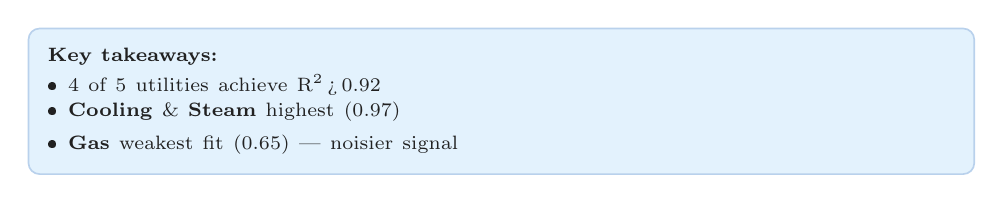
\begin{tikzpicture}
\node[fill=bluelight,rounded corners=4pt,inner sep=7pt,draw=blue1!30,line width=0.6pt,
      text width=0.95\linewidth,align=left]
  {\fontsize{7}{9}\selectfont\textcolor{txtmain}{%
  \textbf{Key takeaways:}\\[2pt]
  \textbullet~4 of 5 utilities achieve R\textsuperscript{2}\,>\,0.92\\
  \textbullet~\textbf{Cooling} \& \textbf{Steam} highest (0.97)\\
  \textbullet~\textbf{Gas} weakest fit (0.65) --- noisier signal%
  }};
\end{tikzpicture}
\end{column}

\end{columns}

\vspace*{\fill}
{\centering\textcolor{txtfaint}{\fontsize{5.5}{7}\selectfont OSU AI Hackathon --- Team Anarchy~~|~~Strategic Energy Investment Prioritization}\par}

\end{frame}
}


% ════════════════════════════════════════════════════════════════
% SLIDE 5: LSTM Gas Model
% ════════════════════════════════════════════════════════════════
{
\begin{frame}[shrink=15]

% Title bar using tikzpicture (not overlay)

\begin{tikzpicture}
\fill[titlebg,rounded corners=3pt] (0,0) rectangle (\textwidth,1.3cm);
\node[anchor=center,font=\Large\bfseries,text=white] at (0.5\textwidth,0.8cm)
  {LSTM Gas Model --- Dual-Branch Architecture};
\node[anchor=center,font=\small,text=white!80] at (0.5\textwidth,0.3cm)
  {GAS\;\textbullet\;1.39M params\;\textbullet\;115 buildings\;\textbullet\;Test R\textsuperscript{2}\,=\,0.9723};
\end{tikzpicture}

\vspace{4pt}

\begin{columns}[T,totalwidth=\textwidth]

% ──── LEFT: Input Features ────
\begin{column}{0.30\textwidth}
\sheader{purple1}{TEMPORAL FEATURES (28)}{1pt}

\flabel{Weather (8)}\\[1pt]
\feat{\textbullet~temperature\_2m}\\
\feat{\textbullet~relative\_humidity\_2m}\\
\feat{\textbullet~dew\_point\_2m}\\
\feat{\textbullet~direct\_radiation}\\
\feat{\textbullet~wind\_speed\_10m}\\
\feat{\textbullet~cloud\_cover}\\
\feat{\textbullet~apparent\_temperature}\\
\feat{\textbullet~precipitation}\\[2pt]

\flabel{Engineered (20)}\\[1pt]
\feat{\textbullet~lag features (1h, 6h, 24h, 1wk)}\\
\feat{\textbullet~rolling mean/std (24h, 1wk)}\\
\feat{\textbullet~cross-utility interactions}\\
\feat{\textbullet~temperature $\times$ area}\\[3pt]

\sheader{deepblue}{STATIC FEATURES (3)}{1pt}
\feat{\textbullet~grossarea\hfill\textcolor{txtfaint}{sqft}}\\
\feat{\textbullet~floorsaboveground\hfill\textcolor{txtfaint}{count}}\\
\feat{\textbullet~building\_age\hfill\textcolor{txtfaint}{years}}\\[4pt]


\begin{tikzpicture}
\node[fill=greenlight,rounded corners=3pt,inner sep=4pt,draw=green1,line width=0.7pt,
      text width=0.9\linewidth,align=center]
  {\textbf{\textcolor{green1}{\small TARGET:~~{\ttfamily energy\_per\_sqft}}}};
\end{tikzpicture}
\end{column}

% ──── MIDDLE: Architecture ────
\begin{column}{0.36\textwidth}
\sheader{orange1}{LSTM BRANCH}{1pt}
\fontsize{7}{9}\selectfont
\renewcommand{\arraystretch}{1.25}
\begin{tabular}{@{}l@{\hspace{8pt}}r@{}}
\textcolor{txtsub}{\ttfamily hidden\_size}    & \textbf{256} \\
\textcolor{txtsub}{\ttfamily num\_layers}     & \textbf{3} \\
\textcolor{txtsub}{\ttfamily dropout}         & \textbf{0.3} \\
\textcolor{txtsub}{\ttfamily bidirectional}   & \textbf{False} \\
\textcolor{txtsub}{\ttfamily max\_grad\_norm} & \textbf{1.0} \\
\textcolor{txtsub}{\ttfamily seq\_length}     & \textbf{48 (12\,hrs)} \\
\textcolor{txtsub}{\ttfamily stride}          & \textbf{4 (1\,hr)} \\
\end{tabular}

\sheader{brown1}{STATIC MLP}{1pt}
\begin{tabular}{@{}l@{\hspace{8pt}}r@{}}
\textcolor{txtsub}{\ttfamily hidden\_dims}    & \textbf{[64]} \\
\textcolor{txtsub}{\ttfamily embedding\_dim}  & \textbf{32} \\
\textcolor{txtsub}{\ttfamily dropout}         & \textbf{0.3} \\
\end{tabular}

\sheader{brown1}{FUSION HEAD}{1pt}
\begin{tabular}{@{}l@{\hspace{8pt}}r@{}}
\textcolor{txtsub}{\ttfamily head\_dims}  & \textbf{[128, 64]} \\
\textcolor{txtsub}{\ttfamily activation}  & \textbf{GELU} \\
\textcolor{txtsub}{\ttfamily dropout}     & \textbf{0.3} \\
\textcolor{txtsub}{\ttfamily input\_dim}  & \textbf{288 (256+32)} \\
\end{tabular}

\vspace{4pt}
% Architecture flow
\centering
\resizebox{0.95\linewidth}{!}{%
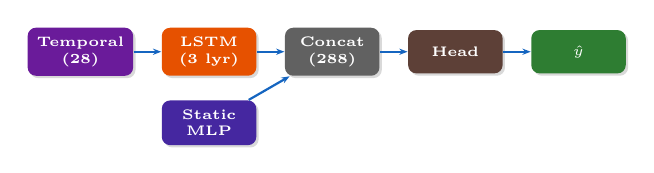
\begin{tikzpicture}[
  node distance=0.35cm,
  block/.style={rectangle,rounded corners=3pt,minimum height=0.55cm,minimum width=1.2cm,
                font=\fontsize{5}{6}\selectfont\bfseries,text=white,align=center,
                drop shadow={shadow xshift=0.3mm,shadow yshift=-0.3mm,opacity=0.3}},
  arr/.style={-{Stealth[length=3pt]},blue1,line width=0.8pt}
]
\node[block,fill=purple1] (temp) {Temporal\\(28)};
\node[block,fill=orange1,right=of temp] (lstm) {LSTM\\(3 lyr)};
\node[block,fill=txtsub,right=of lstm] (cat) {Concat\\(288)};
\node[block,fill=deepblue,below=0.3cm of lstm] (smlp) {Static\\MLP};
\node[block,fill=brown1,right=of cat] (head) {Head};
\node[block,fill=green1,right=of head] (out) {$\hat{y}$};
\draw[arr] (temp) -- (lstm);
\draw[arr] (lstm) -- (cat);
\draw[arr] (smlp) -- (cat);
\draw[arr] (cat) -- (head);
\draw[arr] (head) -- (out);
\end{tikzpicture}%
}
\end{column}

% ──── RIGHT: Training ────
\begin{column}{0.32\textwidth}
\sheader{blue1}{TRAINING CONFIG}{1pt}
\fontsize{7}{9}\selectfont
\renewcommand{\arraystretch}{1.25}
\begin{tabular}{@{}l@{\hspace{8pt}}r@{}}
\textcolor{txtsub}{\ttfamily epochs}          & \textbf{100 (max)} \\
\textcolor{txtsub}{\ttfamily optimizer}       & \textbf{AdamW} \\
\textcolor{txtsub}{\ttfamily learning\_rate}  & \textbf{1e-3} \\
\textcolor{txtsub}{\ttfamily weight\_decay}   & \textbf{1e-4} \\
\textcolor{txtsub}{\ttfamily batch\_size}     & \textbf{512} \\
\textcolor{txtsub}{\ttfamily scheduler}       & \textbf{cosine} \\
\textcolor{txtsub}{\ttfamily early\_stop}     & \textbf{15 epochs} \\
\textcolor{txtsub}{\ttfamily normalize}       & \textbf{z-score} \\
\textcolor{txtsub}{\ttfamily wall\_clock}     & \textbf{33 min (1995s)} \\
\textcolor{txtsub}{\ttfamily gpu}             & \textbf{Tesla T4} \\
\end{tabular}

\vspace{5pt}
% Result box
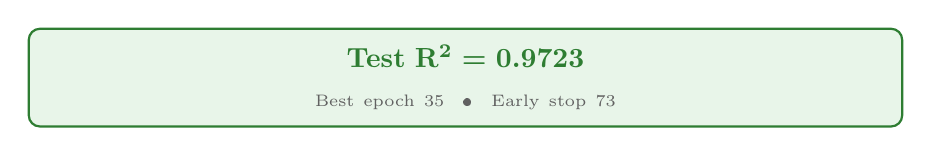
\begin{tikzpicture}
\node[fill=greenlight,rounded corners=4pt,inner sep=6pt,draw=green1,line width=0.8pt,
      text width=0.88\linewidth,align=center]
  {\textbf{\textcolor{green1}{\normalsize Test R\textsuperscript{2} = 0.9723}}\\[2pt]
   \textcolor{txtsub}{\fontsize{6.5}{8}\selectfont Best epoch 35~~\textbullet~~Early stop 73}};
\end{tikzpicture}

\vspace{4pt}

\begin{tikzpicture}
\node[fill=bluelight,rounded corners=3pt,inner sep=4pt,draw=blue1!30,line width=0.5pt,
      text width=0.88\linewidth,align=center]
  {\textcolor{txtsub}{\fontsize{6.5}{8}\selectfont Train: Sep 2025~~|~~Test: Oct 2025}\\
   \textcolor{txtfaint}{\fontsize{6}{7}\selectfont 250K train~~\textbullet~~340K test samples}};
\end{tikzpicture}
\end{column}

\end{columns}

\vspace*{\fill}
{\centering\textcolor{txtfaint}{\fontsize{5.5}{7}\selectfont OSU AI Hackathon --- Team Anarchy~~|~~Strategic Energy Investment Prioritization}\par}

\end{frame}
}


% ════════════════════════════════════════════════════════════════
% SLIDE 6: Gas Model Comparison
% ════════════════════════════════════════════════════════════════
{
\begin{frame}

% Title bar

\begin{tikzpicture}
\fill[titlebg,rounded corners=3pt] (0,0) rectangle (\textwidth,1.3cm);
\node[anchor=center,font=\Large\bfseries,text=white] at (0.5\textwidth,0.8cm)
  {Gas Model Comparison --- 4 Architectures};
\node[anchor=center,font=\small,text=white!80] at (0.5\textwidth,0.3cm)
  {GAS utility~~\textbullet~~Same data split (Sep/Oct 2025)~~\textbullet~~Tesla T4 GPU};
\end{tikzpicture}

\vspace{8pt}

% Main comparison table
\centering
\renewcommand{\arraystretch}{1.8}
\resizebox{0.92\textwidth}{!}{%
\fontsize{10}{13}\selectfont
\begin{tabular}{@{} l
    >{\centering\arraybackslash}p{2.8cm}
    >{\centering\arraybackslash}p{2.8cm}
    >{\centering\arraybackslash}p{2.8cm}
    >{\centering\arraybackslash}p{2.8cm} @{}}
\toprule
\textbf{Metric}
  & \textbf{\textcolor{blue1}{CNN}}
  & \textbf{\textcolor{purple1}{LSTM}}
  & \textbf{\textcolor{orange1}{Transformer}}
  & \textbf{\textcolor{green1}{XGBoost}} \\
\midrule
\textbf{Test R\textsuperscript{2}}
  & \cellcolor{orangelight}\textbf{0.6237}
  & \cellcolor{greenlight}\textbf{0.9723}
  & \cellcolor{greenlight}\textbf{0.9029}
  & \cellcolor{orangelight}\textbf{0.6539} \\
\textbf{Training Time}
  & 8.8 min\newline{\fontsize{8}{10}\selectfont\textcolor{txtfaint}{(525s)}}
  & 33.3 min\newline{\fontsize{8}{10}\selectfont\textcolor{txtfaint}{(1995s)}}
  & 35.9 min\newline{\fontsize{8}{10}\selectfont\textcolor{txtfaint}{(2153s)}}
  & \cellcolor{greenlight}1.7 min\newline{\fontsize{8}{10}\selectfont\textcolor{txtfaint}{(102s)}} \\
\textbf{Parameters}
  & 195K
  & 1.39M
  & 559K
  & 166 trees \\
\textbf{Model Size}
  & 2.3\,MB
  & 5.4\,MB
  & 6.5\,MB
  & \cellcolor{greenlight}151\,KB \\
\bottomrule
\end{tabular}%
}

\vspace{12pt}

% Takeaways
\begin{columns}[T,totalwidth=\textwidth]

\begin{column}{0.48\textwidth}
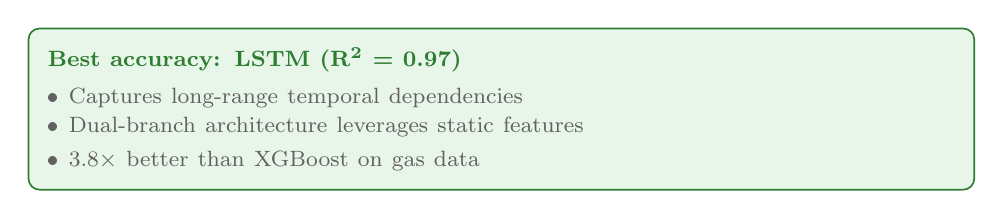
\begin{tikzpicture}
\node[fill=greenlight,rounded corners=4pt,inner sep=7pt,draw=green1,line width=0.6pt,
      text width=0.95\linewidth,align=left] {%
  \fontsize{8}{10.5}\selectfont\textcolor{txtmain}{%
  \textbf{\textcolor{green1}{Best accuracy: LSTM (R\textsuperscript{2} = 0.97)}}\\[3pt]
  \textcolor{txtsub}{%
  \textbullet~Captures long-range temporal dependencies\\
  \textbullet~Dual-branch architecture leverages static features\\
  \textbullet~3.8$\times$ better than XGBoost on gas data}}%
};
\end{tikzpicture}
\end{column}

\begin{column}{0.48\textwidth}
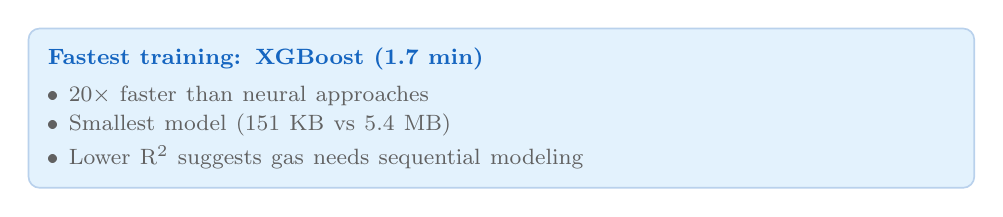
\begin{tikzpicture}
\node[fill=bluelight,rounded corners=4pt,inner sep=7pt,draw=blue1!30,line width=0.6pt,
      text width=0.95\linewidth,align=left] {%
  \fontsize{8}{10.5}\selectfont\textcolor{txtmain}{%
  \textbf{\textcolor{blue1}{Fastest training: XGBoost (1.7 min)}}\\[3pt]
  \textcolor{txtsub}{%
  \textbullet~20$\times$ faster than neural approaches\\
  \textbullet~Smallest model (151 KB vs 5.4 MB)\\
  \textbullet~Lower R\textsuperscript{2} suggests gas needs sequential modeling}}%
};
\end{tikzpicture}
\end{column}

\end{columns}

\vspace*{\fill}
{\centering\textcolor{txtfaint}{\fontsize{5.5}{7}\selectfont OSU AI Hackathon --- Team Anarchy~~|~~Strategic Energy Investment Prioritization}\par}

\end{frame}
}

\end{document}
